% Copyright (c) 2022 Tobias Briones. All rights reserved.
%
% SPDX-License-Identifier: CC-BY-SA-4.0
%
% This file is part of Course Project at UNAH-IS911: Microprocessors.
%
% This source code is licensed under the Creative Commons Attribution Share
% Alike 4.0 International License found in the LICENSE file in the root
% directory of this source tree or at https://spdx.org/licenses/CC-BY-SA-4.0.

\documentclass{article}
\usepackage{preamble}

\title{LAB 2: LDR PARA MEDIR LA LUZ}
\author{Tobias Briones \bigbreak tobias.briones@unah.hn}
\date{Septiembre 2021}

\begin{document}

    \makeatletter
    \begin{titlepage}
        \begin{center}
            
\includegraphics[width=0.3\linewidth]{images/logo-unah}\\[4ex]
            {\huge \bfseries \@title
            \vspace{1cm}}\\[2ex]
            {\LARGE \@author}\\[50ex]

            {\large
            Universidad Nacional Autónoma de Honduras\\
            Ingeniería de Sistemas\\
            I PAC 2022\\
            IS911-MICROPROCESADORES
            }\\[2ex]

            {\large \today}
        \end{center}
    \end{titlepage}
    \makeatother
    \thispagestyle{empty}
    \newpage

    \import{}{footer}

    \section{Objetivos}

    \subsection{Objetivo General}

    Depurar el valor análogo de un LDR mediante el serial de Arduino y el
    simulador Proteus.

    \subsection{Objetivos Específicos}

    \begin{itemize}
        \item Crear un programa Arduino que mida y depure por Serial el valor
        de un LDR básico.
        \item Crear el circuito correspondiente en Proteus para correr el
        programa.
        \item Entender el uso de la foto-resistencias y lectura de señales
        analógicas básicas del Arduino.
    \end{itemize}

    \section{Marco Teórico}

    Para el desarrollo de este laboratorio se necesita comprender conceptos
    básicos sobre foto-resistencias y señales análogas en Arduino.

    \subsection{Señales Analógicas}

    Al emplear sensores digitales las variables obviamente son cero o uno, es
    decir, valores binarios o digitales o discretos donde un cero puede
    equivales a $0v$ y un uno a $1v$. Con respecto a señales analógicas
    tenemos valores continuos en el intervalo $[0, 5]v$. El Arduino UNO tiene
    6 puertos análogos que son los puertos $A_0 - A_5$ y la resolución del
    Arduino es de $10 bit$ por lo que se puede tener un valor máximo de
    $2^{10} = 1024 \, bit$ de lectura \cite{flores-2018}.

    \bigbreak

    Por lo que se puede calcular el valor que interesa de la siguiente manera

    $$
    V = \frac{V_{analog}}{2^{n-1}} V_{ref}
    $$

    Luego también se pueden hacer transformaciones de los valores útiles,
    como por ejemplo, convertir la lectura de $[0, 1023]$ al intervalo $[0,
    255]$ mediante el método $map$. Sea $A = [a_1, a_2]$ el intervalo
    original y $B = [b_1, b_2]$ el intervalo destino. Entonces la firma de la
    función map es $map(valor, \, a_1, \, a_2, \, b_1, \, b_2)$.

    \bigbreak

    Por último, también se encuentran aplicaciones del transistor para
    control de potencia, opto-acopladores en la sección $4.4$ y comunicación
    mediante el Serial de Arduino en la sección $4.6$ de \textit{Curso Básico
    de Arduino} \cite{flores-2018}.

    \subsection{Comunicación con el Serial}

    De acuerdo a la documentación, la API Serial de Arduino:

    \begin{quote}
        Se utiliza para la comunicación entre la placa Arduino y una
        computadora u otros dispositivos. Todas las placas Arduino tienen al
        menos un puerto serie (también conocido como UART o USART), y algunas
        tienen varios.\\ \footnotesize
        Fuente: Arduino $\mid$ Serial - Arduino Reference (traducido de
        inglés a español) \cite{arduino-serial}
    \end{quote}

    También menciona que los pines $0,1$ deberían ser usados para la
    comunicación en la mayoría de los modelos de Arduino y en caso de haber
    otra conexión en esos puertos entonces la comunicación es interferida.
    También puede ser necesario un cable USB a Serial para establecer la
    conexión con el ordenador.

    \bigbreak

    El método $begin$ se utiliza en el método $setup$ para crear la
    comunicación y luego otros métodos como $read$ se utilizan para obtener
    los datos en el loop. El método $begin$ recibe como argumento la
    velocidad de transferencia de datos en bits por segundo (baudios).

    \bigbreak

    \begin{lstlisting}[language=C, caption=Uso de Serial en Arduino Mega con
    todos sus puertos Seriales. \footnotesize Fuente: Serial - Arduino
    Reference (begin) \cite{arduino-serial}]
    void setup()
    {
        Serial.begin(9600);
        Serial1.begin(38400);
        Serial2.begin(19200);
        Serial3.begin(4800);

        Serial.println("Hello Computer");
        Serial1.println("Hello Serial 1");
        Serial2.println("Hello Serial 2");
        Serial3.println("Hello Serial 3");
    }
\end{lstlisting}


\begin{lstlisting}[language=C, caption=Uso del método read. \footnotesize
Fuente: Serial - Arduino Reference (read) \cite{arduino-serial}]
int incomingByte = 0; // for incoming serial data

void setup()
{
    Serial.begin(9600); // opens serial port, sets data rate to 9600 bps
}

void loop()
{
    // send data only when you receive data:
    if (Serial.available() > 0)
    {
        // read the incoming byte:
        incomingByte = Serial.read();

        // say what you got:
        Serial.print("I received: ");
        Serial.println(incomingByte, DEC);
    }
}
\end{lstlisting}

\subsection{Lectura analógica}

Según la documentación, la lectura de señales analógicas mediante el método
$analogRead$:

\begin{quote}
Lee el valor del pin analógico especificado. Las tarjetas Arduino contienen
un convertidor analógico a digital multicanal de 10 bits. Esto significa que
mapeará los voltajes de entrada entre 0 y el voltaje de funcionamiento (5v o
3.3v) en valores enteros entre 0 y 1023. En un Arduino UNO, por ejemplo, esto
produce una resolución entre lecturas de: 5 voltios / 1024 unidades o , 0
.0049 voltios (4.9mV) por unidad. \\ \footnotesize
Fuente: Arduino $\mid$ analogRead() - Arduino Reference (traducido de inglés
a español) \cite{arduino-analogRead}
\end{quote}

El cual se puede usar de la siguiente manera:

\begin{lstlisting}[language=C, caption=Uso del método analogRead.
\footnotesize Fuente: analogRead() - Arduino Reference
\cite{arduino-analogRead}]
int analogPin = A3; // potentiometer wiper (middle terminal) connected to
// analog pin 3
// outside leads to ground and +5V
int val = 0;  // variable to store the value read

void setup()
{
    Serial.begin(9600);           //  setup serial
}

void loop()
{
    val = analogRead(analogPin);  // read the input pin
    Serial.println(val);          // debug value
}
\end{lstlisting}

\subsection{Fotoresistencia (LDR)}

En esta sección se establece que es una fotoresistencia o light-dependent
resistor (LDR). Este es un dispositivo sensor que simplemente transforma la
luz que recibe en una valor de resistencia. Se puede usar para encender una
luz al anochecer por ejemplo.

\bigbreak

Según Wikipedia, la definición de una fotoresistencia es:

\begin{quote}
Una fotorresistencia (también conocida como fotocélula, resistencia
dependiente de la luz, LDR o célula fotoconductora) es un componente pasivo
que reduce la resistencia con respecto a la recepción de luminosidad (luz) en
la superficie sensible del componente. La resistencia de un fotoresistor
disminuye con el aumento de la intensidad incidente; en otras palabras,
exhibe fotoconductividad.\\ \footnotesize
Fuente: Wikipedia $\mid$ Photoresistor (traducido de inglés a español)
\cite{wikipedia-ldr-2022}
\end{quote}

Además también pueden ser utilizadas para aplicaciones de seguridad que
detectan cuando pasa un objeto o persona al tapar la luz que emite un laser.

\bigbreak

Estos sensores lucen de la siguiente manera:

\begin{figure}[H]
\centering
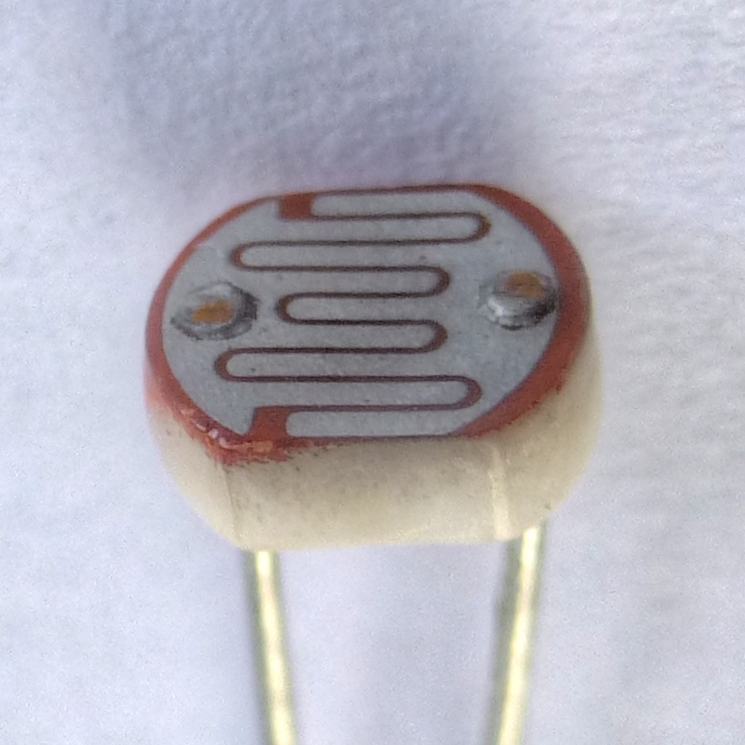
\includegraphics[width=0.2\paperwidth]{images/ldr.jpg}
\caption{Fotoresistor}\footnotesize
Fuente: \textit{Wikipedia $\mid$ Photoresistor} \cite{wikipedia-ldr-2022}. By
© Nevit Dilmen, CC BY-SA 3.0, https://commons.wikimedia.org/w/index
.php?curid=30560805.
\end{figure}

\begin{figure}[H]
\centering
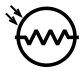
\includegraphics[width=0.2\paperwidth]{images/ldr-symbol}
\caption{Símbolo de un Fotoresistor}\footnotesize
Fuente: \textit{Wikipedia $\mid$ Photoresistor} \cite{wikipedia-ldr-2022}. By
User:FDominec et al. - File:Electrical\_symbols\_library.svg, CC0,
https://commons.wikimedia.org/w/index.php?curid=49516462.
\end{figure}

\begin{figure}[H]
\centering
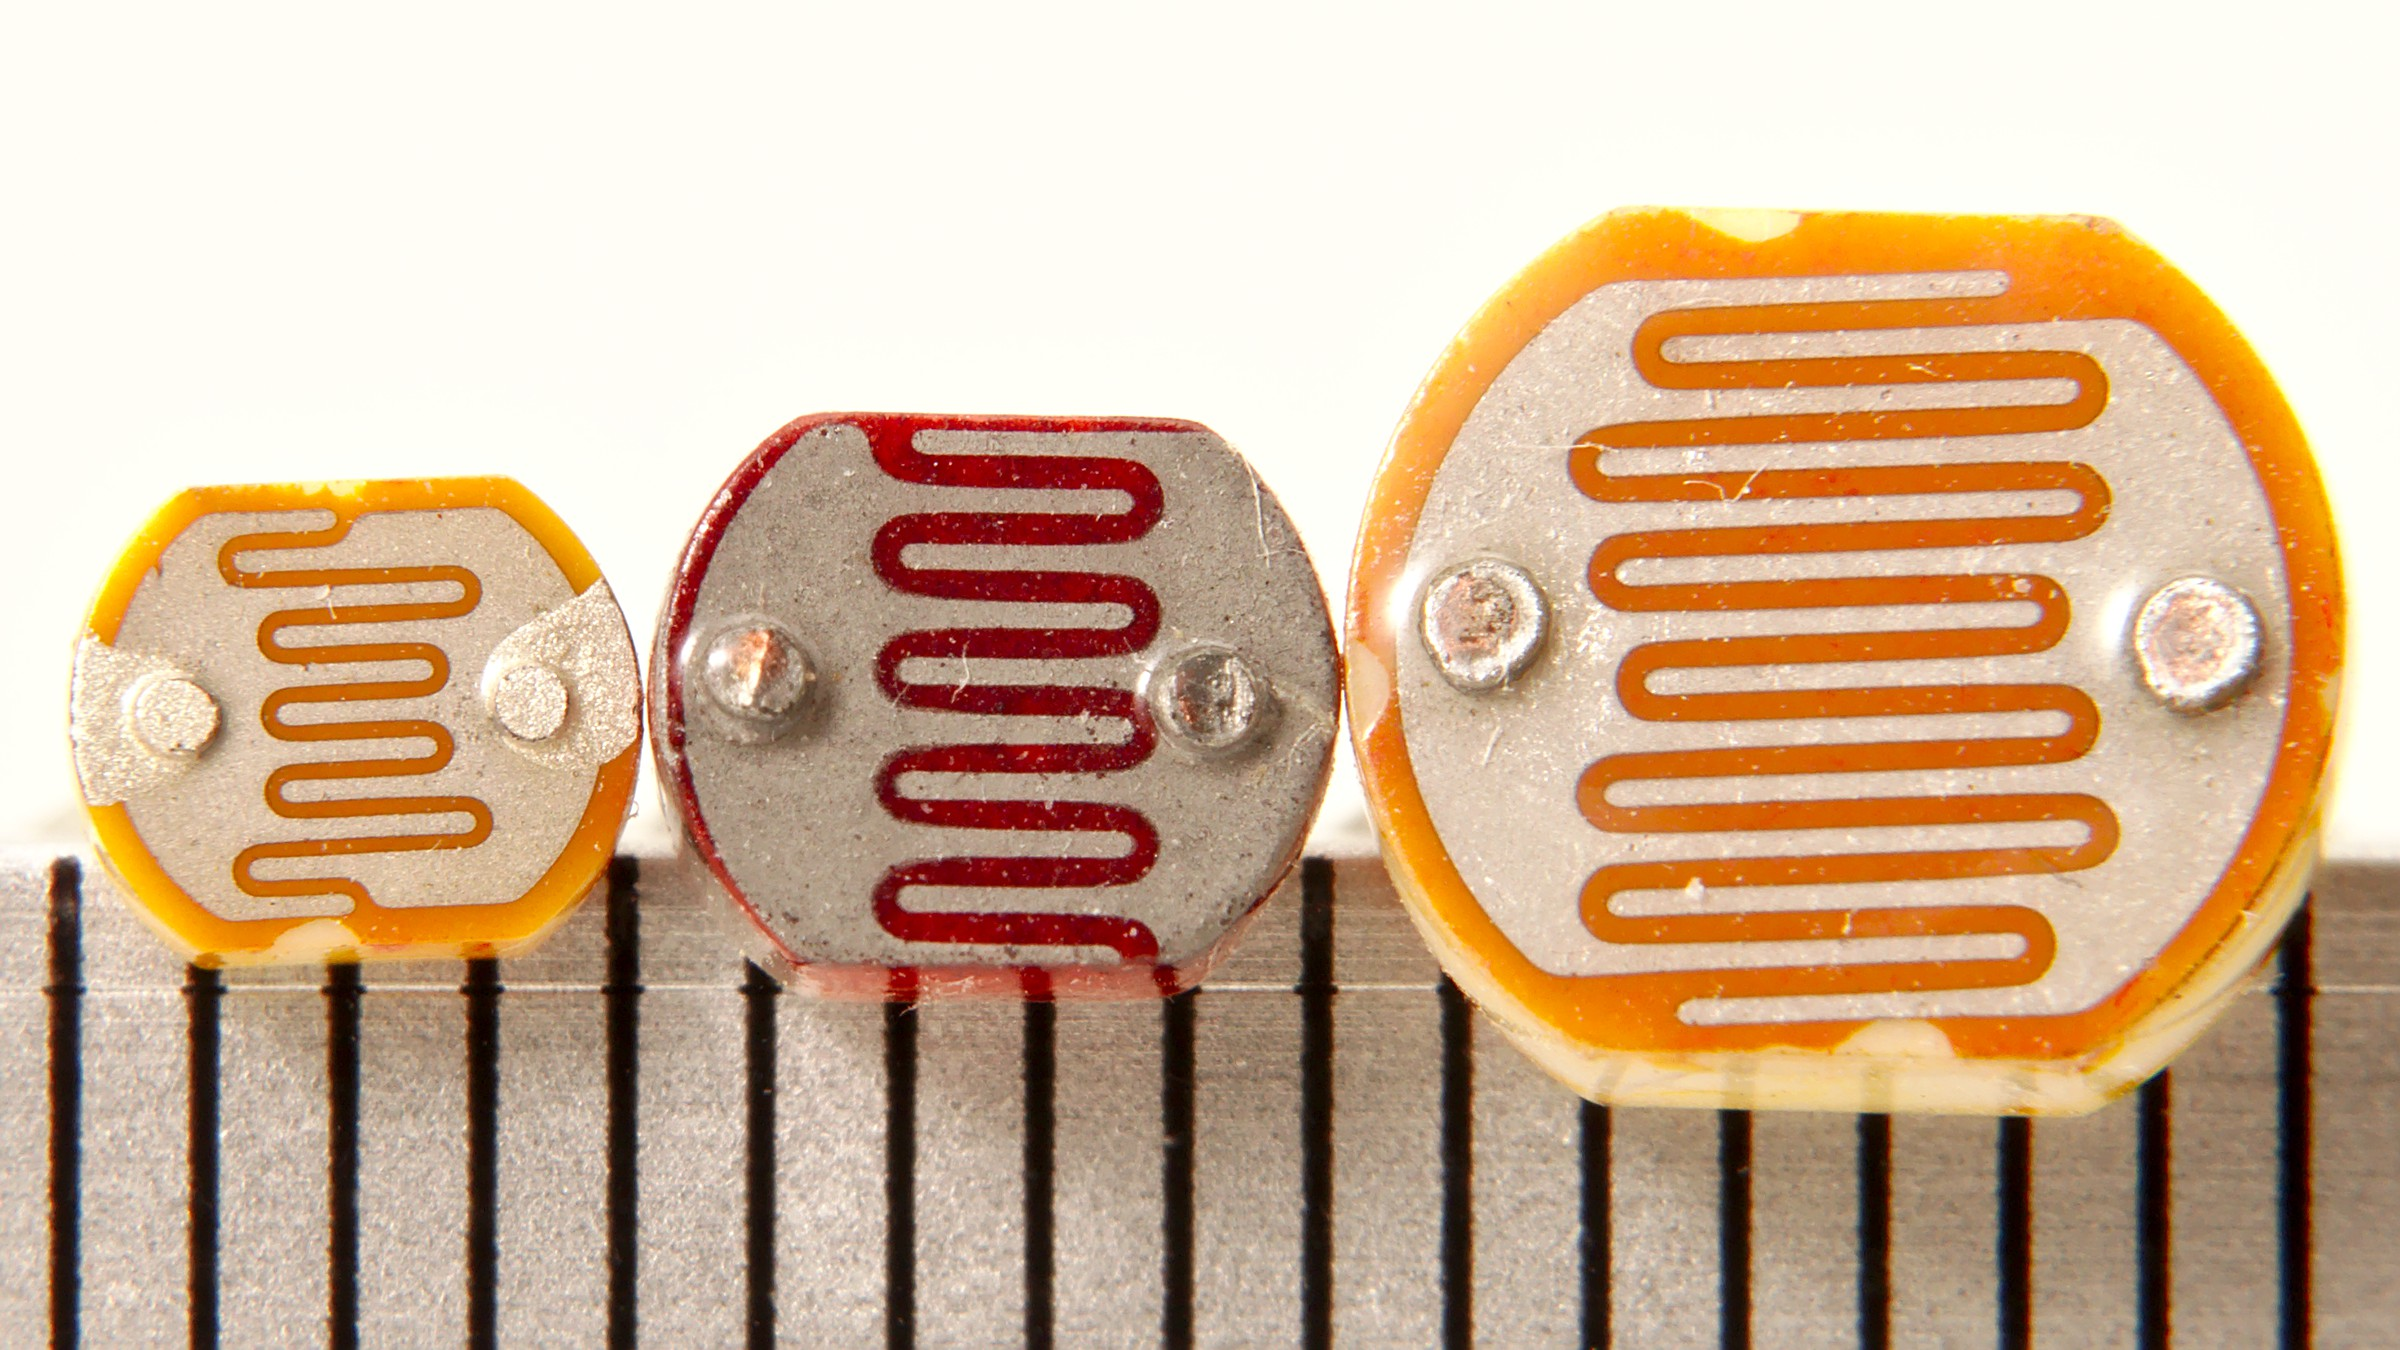
\includegraphics[width=0.2\paperwidth]{images/ldr-three-sizes.jpg}
\caption{Fotoresistores en tres tamaños}\footnotesize
Fuente: \textit{Wikipedia $\mid$ Photoresistor} \cite{wikipedia-ldr-2022}. By
Junkyardsparkle - Own work, CC0, https://commons.wikimedia.org/w/index
.php?curid=35977178.
\end{figure}

\section{Procedimiento Experimental}

\subsection{Programa Arduino}

Para crear el programa en Arduino IDE primero se declara una variable $ldr$
para indicar el puerto del sensor LDR el cual será medido en el puerto $0$.
Recordar que debería de ser puerto $0$ o $1$.

\bigbreak

En el $setup$ se establece el pin del LDR y se inicializa el Serial a una
velocidad de $9,600$ baudios de datos.

\bigbreak

Por último, se lee la entrada análoga del sensor con el método $analogRead$,
se imprime el valor por el Serial y se espera $1$ segundo para dar chance al
sistema.

\begin{figure}[H]
\centering
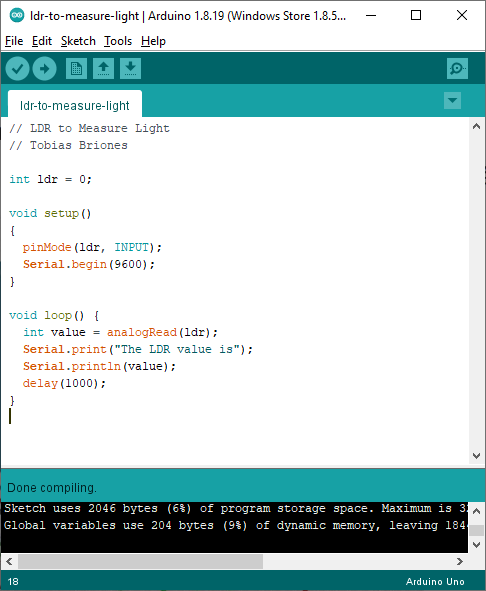
\includegraphics[width=0.3\paperwidth]{images/arduino-sketch}
\caption{Programa Arduino}\footnotesize
\textit{Derivative screenshot from Arduino IDE under fair use}
\end{figure}

Para terminar se compila el código para su verificación en el botón
\say{Verificar} y se guarda el binario con el bootloader para que sea cargado
a Proteus en \say{Sketch - Export compiled binary}.

\subsection{Simulación}

Para hacer la simulación es posible hacerla de la forma sencilla como en el
laboratorio 1 o instalando la librería de Arduino (SIMULINO) el cual consiste
en solo copiar los archivos al directorio de instalación de Proteus. Se usará
la segunda opción.

\bigbreak

Crear un nuevo proyecto y seleccionar las opciones por defecto. Agregar y
conectar como se muestra en el diagrama abajo los siguientes dispositivos:

\begin{itemize}
\item Arduino UNO
\item Resistencia (10K)
\item LDR (con foquito)
\end{itemize}

\begin{figure}[H]
\centering
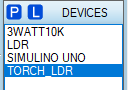
\includegraphics[width=0.1\paperwidth]{images/proteus-devices}
\caption{Dispositivos a agregar}\footnotesize
\textit{Derivative screenshot from Proteus under fair use}
\end{figure}

Al hacer la conexión del circuito faltará agregar la \say{Terminal virtual}
que se encuentra en el menú \say{Virtual Instruments Mode} de Proteus.

\begin{figure}[H]
\centering
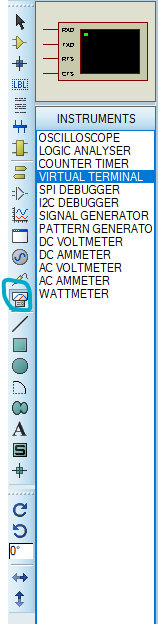
\includegraphics[width=0.1\paperwidth]{images/proteus-virtual-terminal}
\caption{Agregar terminal virtual}\footnotesize
\textit{Derivative screenshot from Proteus under fair use}
\end{figure}

Por último se corre la simulación.

\begin{figure}[H]
\centering
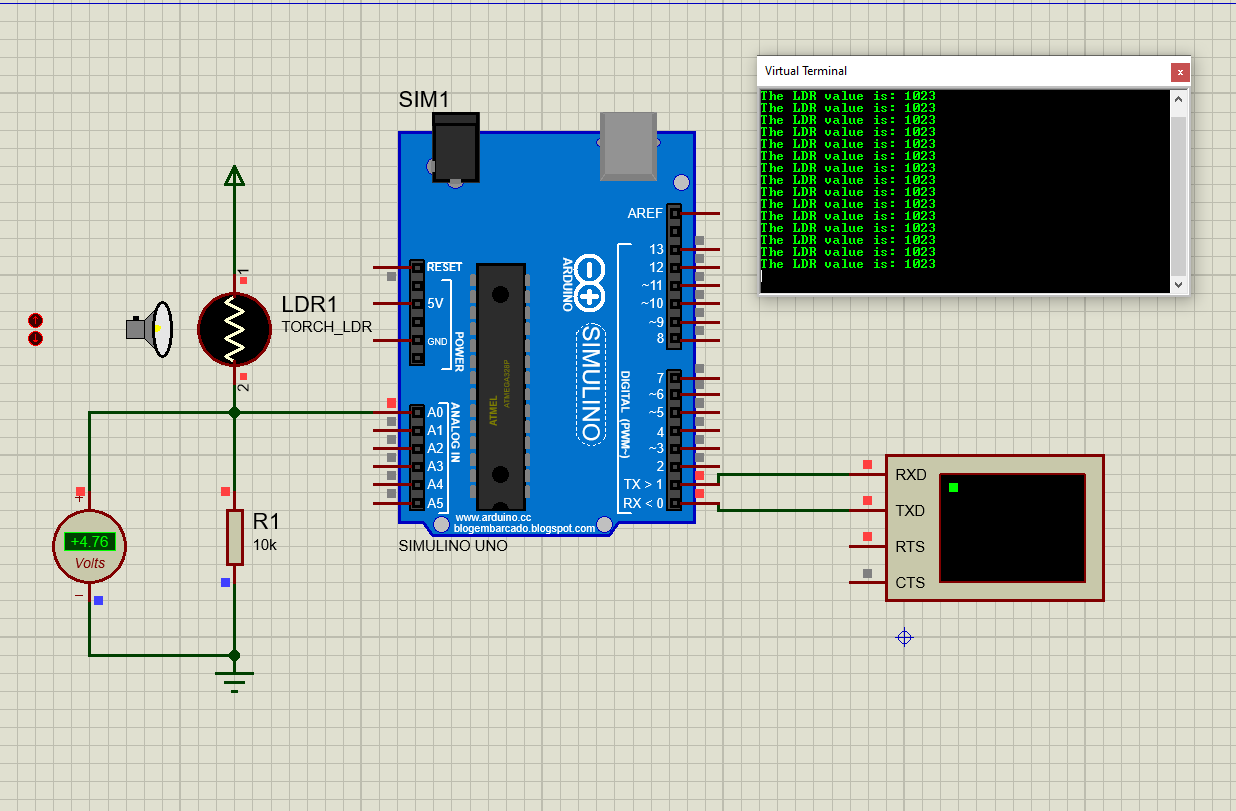
\includegraphics[width=0.3\paperwidth]{images/sim-1}
\caption{Simulación en Proteus}\footnotesize
\textit{Derivative screenshot from Proteus under fair use}
\end{figure}

Y se verifica con un voltímetro de corriente directa el divisor de tensión el
cual cambia su resistencia cuando se cambia la luminosidad de la
fotoresistencia.

\begin{figure}[H]
\centering
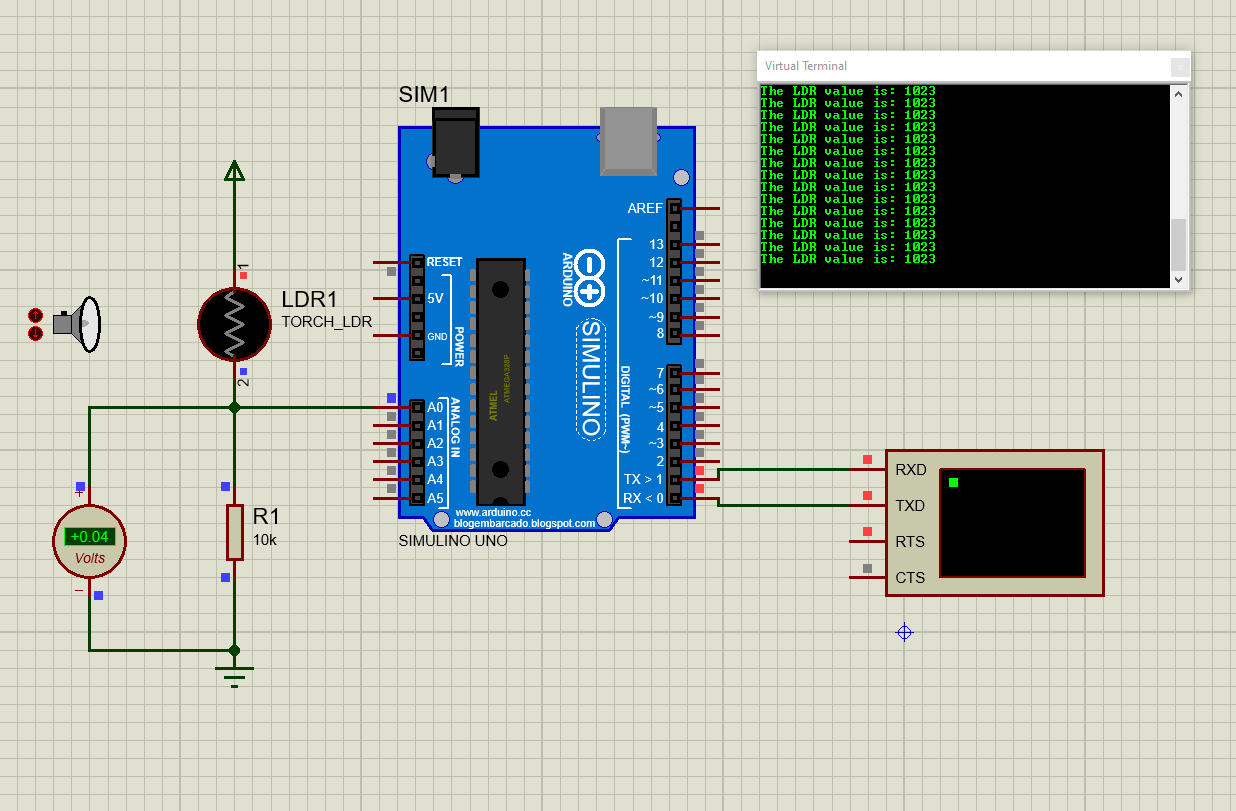
\includegraphics[width=0.3\paperwidth]{images/sim-2}
\caption{Verificación del divisor de tensión}\footnotesize
\textit{Derivative screenshot from Proteus under fair use}
\end{figure}

Sin embargo no fue posible que el Arduino tomara los valores de $A0$ a pesar
de estar el circuito y el programa bien y haber intentado varias formas
diferentes.

\section{Análisis de Resultados}

El valor del puerto $A0$ del Arduino es proporcional al la cantidad de luz
que incide sobre la fotoresistencia. Se probó que cuando la iluminación es
máxima hay $+4.76V$ en $A0$ y cuando es mínima el valor es de $+0.04V$ el
cual varía proporcionalmente a la variación de la fuente de luz. La salida
Serial del Arduino debió haber leído estos valores que obtuvo el voltímetro
pero no fue posible por alguna razón de la simulación y solo mostraba $1023$
el valor máximo de forma constante.

\section{Conclusión}

Se desarrolló un programa en Arduino que lee la entrada análoga de una
fotoresistencia e imprime el valor por la salida Serial y se simuló el
circuito en Proteus comprobando el funcionamiento del divisor de tensión con
un voltímetro de corriente directa. También se tuvo que agregar una terminal
virtual para leer el Serial del Arduino y se utilizó la versión
\say{colorida} de la tarjeta Arduino para la simulación en Proteus.

\printbibliography

\end{document}
